\documentclass{article}\usepackage{graphicx, color}
%% maxwidth is the original width if it is less than linewidth
%% otherwise use linewidth (to make sure the graphics do not exceed the margin)
\makeatletter
\def\maxwidth{ %
  \ifdim\Gin@nat@width>\linewidth
    \linewidth
  \else
    \Gin@nat@width
  \fi
}
\makeatother

\definecolor{fgcolor}{rgb}{0.2, 0.2, 0.2}
\newcommand{\hlnumber}[1]{\textcolor[rgb]{0,0,0}{#1}}%
\newcommand{\hlfunctioncall}[1]{\textcolor[rgb]{0.501960784313725,0,0.329411764705882}{\textbf{#1}}}%
\newcommand{\hlstring}[1]{\textcolor[rgb]{0.6,0.6,1}{#1}}%
\newcommand{\hlkeyword}[1]{\textcolor[rgb]{0,0,0}{\textbf{#1}}}%
\newcommand{\hlargument}[1]{\textcolor[rgb]{0.690196078431373,0.250980392156863,0.0196078431372549}{#1}}%
\newcommand{\hlcomment}[1]{\textcolor[rgb]{0.180392156862745,0.6,0.341176470588235}{#1}}%
\newcommand{\hlroxygencomment}[1]{\textcolor[rgb]{0.43921568627451,0.47843137254902,0.701960784313725}{#1}}%
\newcommand{\hlformalargs}[1]{\textcolor[rgb]{0.690196078431373,0.250980392156863,0.0196078431372549}{#1}}%
\newcommand{\hleqformalargs}[1]{\textcolor[rgb]{0.690196078431373,0.250980392156863,0.0196078431372549}{#1}}%
\newcommand{\hlassignement}[1]{\textcolor[rgb]{0,0,0}{\textbf{#1}}}%
\newcommand{\hlpackage}[1]{\textcolor[rgb]{0.588235294117647,0.709803921568627,0.145098039215686}{#1}}%
\newcommand{\hlslot}[1]{\textit{#1}}%
\newcommand{\hlsymbol}[1]{\textcolor[rgb]{0,0,0}{#1}}%
\newcommand{\hlprompt}[1]{\textcolor[rgb]{0.2,0.2,0.2}{#1}}%

\usepackage{framed}
\makeatletter
\newenvironment{kframe}{%
 \def\at@end@of@kframe{}%
 \ifinner\ifhmode%
  \def\at@end@of@kframe{\end{minipage}}%
  \begin{minipage}{\columnwidth}%
 \fi\fi%
 \def\FrameCommand##1{\hskip\@totalleftmargin \hskip-\fboxsep
 \colorbox{shadecolor}{##1}\hskip-\fboxsep
     % There is no \\@totalrightmargin, so:
     \hskip-\linewidth \hskip-\@totalleftmargin \hskip\columnwidth}%
 \MakeFramed {\advance\hsize-\width
   \@totalleftmargin\z@ \linewidth\hsize
   \@setminipage}}%
 {\par\unskip\endMakeFramed%
 \at@end@of@kframe}
\makeatother

\definecolor{shadecolor}{rgb}{.97, .97, .97}
\definecolor{messagecolor}{rgb}{0, 0, 0}
\definecolor{warningcolor}{rgb}{1, 0, 1}
\definecolor{errorcolor}{rgb}{1, 0, 0}
\newenvironment{knitrout}{}{} % an empty environment to be redefined in TeX

\usepackage{alltt}
\usepackage{mathtools}
\usepackage{amsfonts}
\usepackage{float}
\usepackage{graphicx}
\usepackage{caption}
\usepackage{Sweave,bbm,amsmath,url}
\usepackage{subcaption}
\IfFileExists{upquote.sty}{\usepackage{upquote}}{}

\begin{document}
\title{Random Portfolios}
\author{Mike Flynn, Angel Zhou, Dave Kane}
\maketitle

\section*{Introduction}




Put yourself in a scenario where you have 6,250 dollars. Let's say that you want to invest this money in two stocks: General Electric (GE) and International Business Machines (IBM). There is an endless number of ways that you could split your money into the two stocks. For example, you could invest 25 percent of your 6,250 dollars in GE and the remaining 75 percent in IBM. In another scenario, you could halve your money by putting 3,125 dollars into GE and 3,125 dollars into IBM. The possibilities stretch on.

\begin{figure}[H]
  \begin{subfigure}[b]{0.5\textwidth}
      \centering
      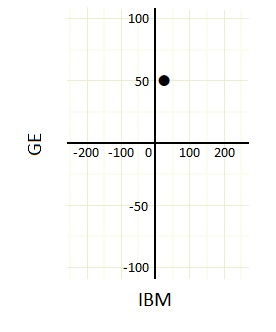
\includegraphics[width=\textwidth]{sharespace}
      \label{fig:sharespace}
  \end{subfigure}
  \begin{subfigure}[b]{0.5\textwidth}
      \centering
      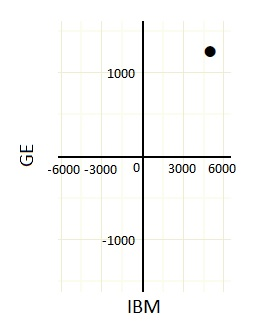
\includegraphics[width=\textwidth]{dollarspace}
      \label{fig:dollarspace}
      \end{subfigure}
\caption{Consider the situation where you invest in 25 shares of IBM and 50 shares of GE. This coordinate, where $x = 25$ and $y = 50$, is displayed on the left plot. This graph thus shows a single portfolio in what is called a share space, meaning that the x and y coordinates represent the amount of shares invested in each stock. Alternatively, one can view the portfolio in dollar terms. This is done by multiplying the stock price by the number of shares, resulting in the total amount spent in each stock. The price of GE is currently at around 25 dollars apiece while the value of each IBM stock is approximately 200 dollars. Thus, 25 shares of IBM becomes 5,000 dollars and 50 shares of GE costs 1,250 dollars. The plot on the right displays the same portfolio as the one on the left, but plots the portfolio in dollar space. This means that the x and y coordinates represent the amount of money that is invested into each respective stock.}
\end{figure}

Now that we have seen portfolios in both share and dollar space, what else is there?
\\
\\
Portion space refers to percentages. Say you spend 30 percent of your money on IBM. In other words, .3 of your total money is invested in IBM. For the rest of this document, we will be referring to portfolios plotted in portion space.

\begin{figure}[H]
  \begin{subfigure}[b]{1.0\textwidth}
    \centering
    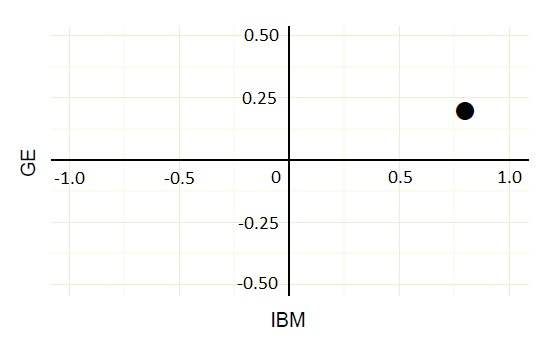
\includegraphics[width=\textwidth]{portionspace}
    \label{fig:portionspace}
  \end{subfigure}
\caption{The same portfolio as that in Figure 1 is considered again in the above plot. Instead of share or dollar space, the portfolio (consisting of 25 and 50 shares of IBM and GE respectively) is now shown in portion space. Given that you hypothetically invest 5,000 dollars on IBM and 1,250 dollars on GE, you expend a total of 6,250 dollars (since all of your money was spent, this portfolio is fully invested; no money is put aside for other purposes). $1250/6250 = 0.2$, so 20 percent of your budget is spent in GE. Transitively, 80 percent is put into IBM. These percentages are plotted as decimals.}
\end{figure}

As mentioned before, there is an infinite number of ways to split the invested money. No matter how you divide your total dollar amount, whether you put .5 in IBM and .5 in GE, or .2 in IBM and .8 in GE, the two values must sum to 1, or 100 percent. In other words, every portfolio that we will consider will be fully invested.
\\
\\
In order to visualize how all the possible portfolios would appear in a 2-D space, you can generate random weights, creating a completely arbitrary way of splitting the money. Some constraints that must be followed when generating random weights are as follows: $x + y = 1$ and ${x, y} > 0$.

\begin{figure}[H]
  \begin{subfigure}[b]{0.7\textwidth}
      \centering
      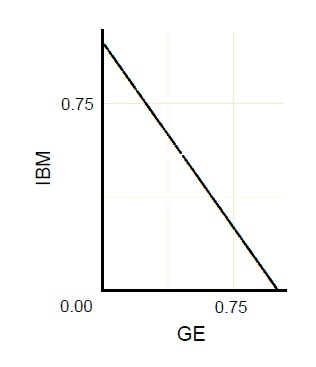
\includegraphics[width=\textwidth]{samples}
      \label{fig:samples}
  \end{subfigure}
\caption{1,000 random samples of General Electric (GE) and International Business Machines (IBM) are taken. Each point represents a possible portfolio. The result is a diagonal line extending from the point (0,1) to the point (1,0). Because x and y must sum to 1, a line is formed where every set of x and y coordinates add up to 1.}
\end{figure}

Let's say that you want to add Coca-Cola (KO) to the stocks that you are investing in. Now that you have three stocks instead of two, you must generate three random weights that sum to 1. To create an example, you could invest .3, .3, and .4 of your total funding in KO, GE, and IBM respectively. 
  
\begin{figure}[H]
\begin{knitrout}
\definecolor{shadecolor}{rgb}{0.969, 0.969, 0.969}\color{fgcolor}
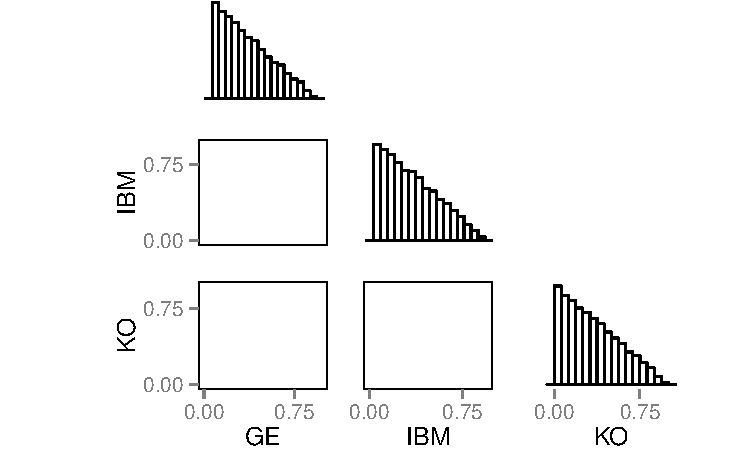
\includegraphics[width=\maxwidth]{figure/figChunk1} 

\end{knitrout}

\caption{1,000 random weights were sampled for Google (GE), Coca-Cola (KO), and International Business Machines (IBM). Once again, these portfolios are all fully invested. The pairwise scatterplots display the same distribution of the 1,000 random weights. According to the plots, the maximum sum for the weight distributions for any two variables is 1, and the minimum sum is 0.
\\
\\
The three histograms on the diagonal represent density plots of 10,000 randomly sampled weights. More samples are taken for the histograms in order to increase their resolution. The histograms display the distributions of the variables and they indicate that the most likely value for any given variable is close to 0.}

\end{figure}

Now let's consider yet another scenario, where you are investing in five different stocks: General Electric (GE), International Business MAchines (IBM), Coca-Cola (KO), General Motors (GM), and Microsoft (MSFT). Like before, the generated portfolios are fully invested. For example, one possible portfolio could consist of the weights 0.2, 0.3, 0.1, 0.15, 0.25 for each respective stock.

\begin{figure}[H]
\begin{knitrout}
\definecolor{shadecolor}{rgb}{0.969, 0.969, 0.969}\color{fgcolor}

\includegraphics[width=\maxwidth]{figure/fiveByFiveGrid} 

\end{knitrout}

\end{figure}

\begin{figure}[H]
  \begin{subfigure}[b]{1.0\textwidth}
    \centering
    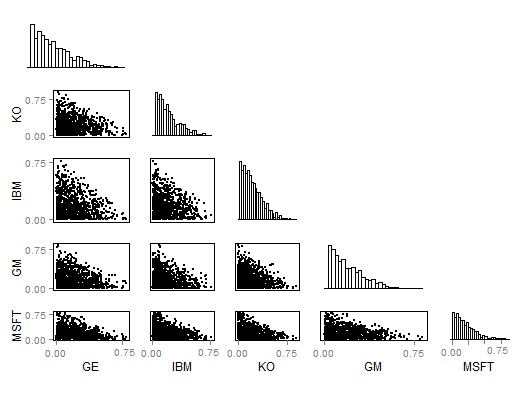
\includegraphics[width=\textwidth]{5v5}
    \label{fig:5v5}
  \end{subfigure}
\caption{1,000 random weights were sampled for Google (GE), Coca-Cola (KO), International Business Machines (IBM), General Motors (GM), and Microsoft (MSFT).
\\
\\
10,000 weights were randomly sampled for the five histograms. These graphs function as density plots.}
\end{figure}

\section*{hitandrun()}

In order to create the scatterplots and histograms previously shown in this document, random points had to be generated. These points were created using a function called hitandrun(). The algorithm for this function requires several steps:

\begin{figure}[H]
\begin{knitrout}
\definecolor{shadecolor}{rgb}{0.969, 0.969, 0.969}\color{fgcolor}
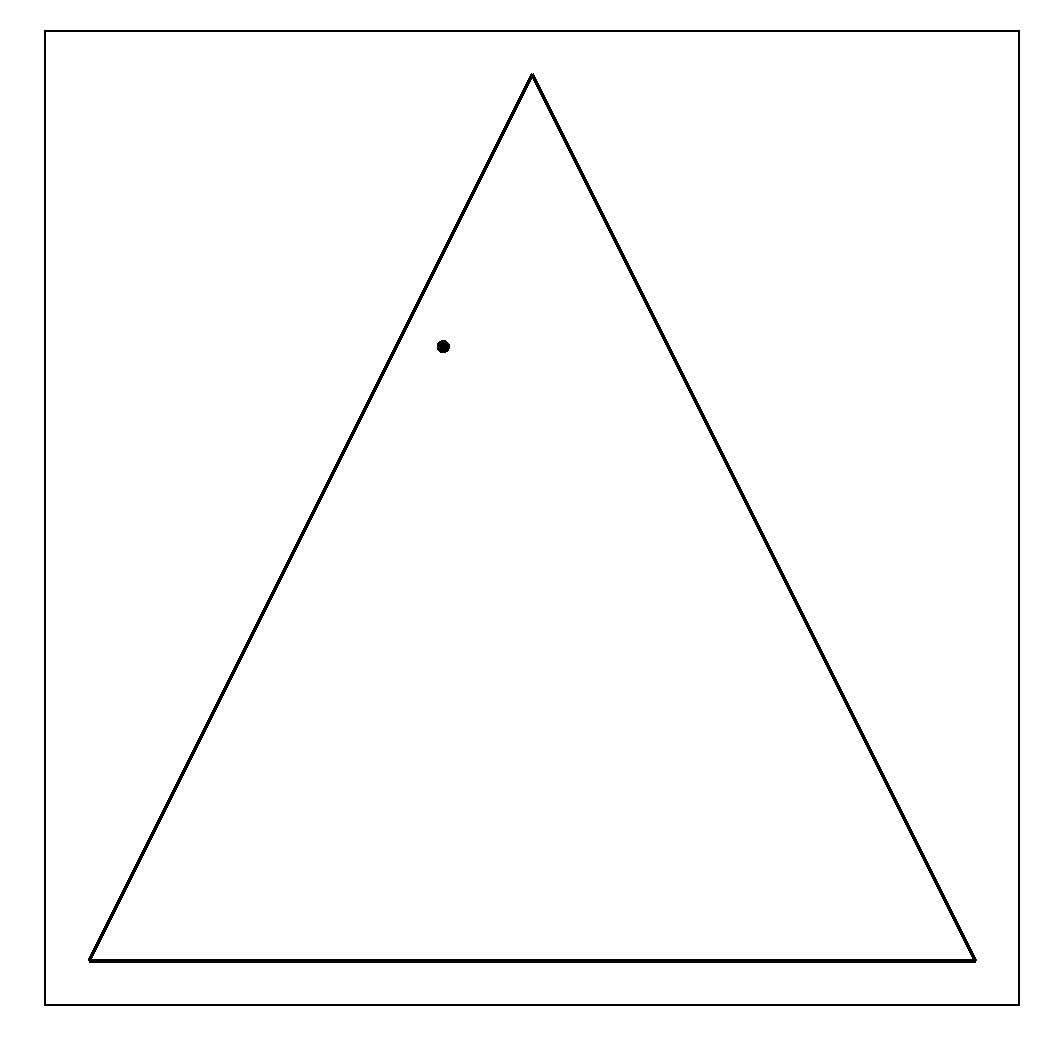
\includegraphics[width=\maxwidth]{figure/hitandrun_walkthrough1} 

\end{knitrout}

\caption{hitandrun() first picks a random point within a simplex.}
\end{figure}

\begin{figure}[H]
\begin{knitrout}
\definecolor{shadecolor}{rgb}{0.969, 0.969, 0.969}\color{fgcolor}
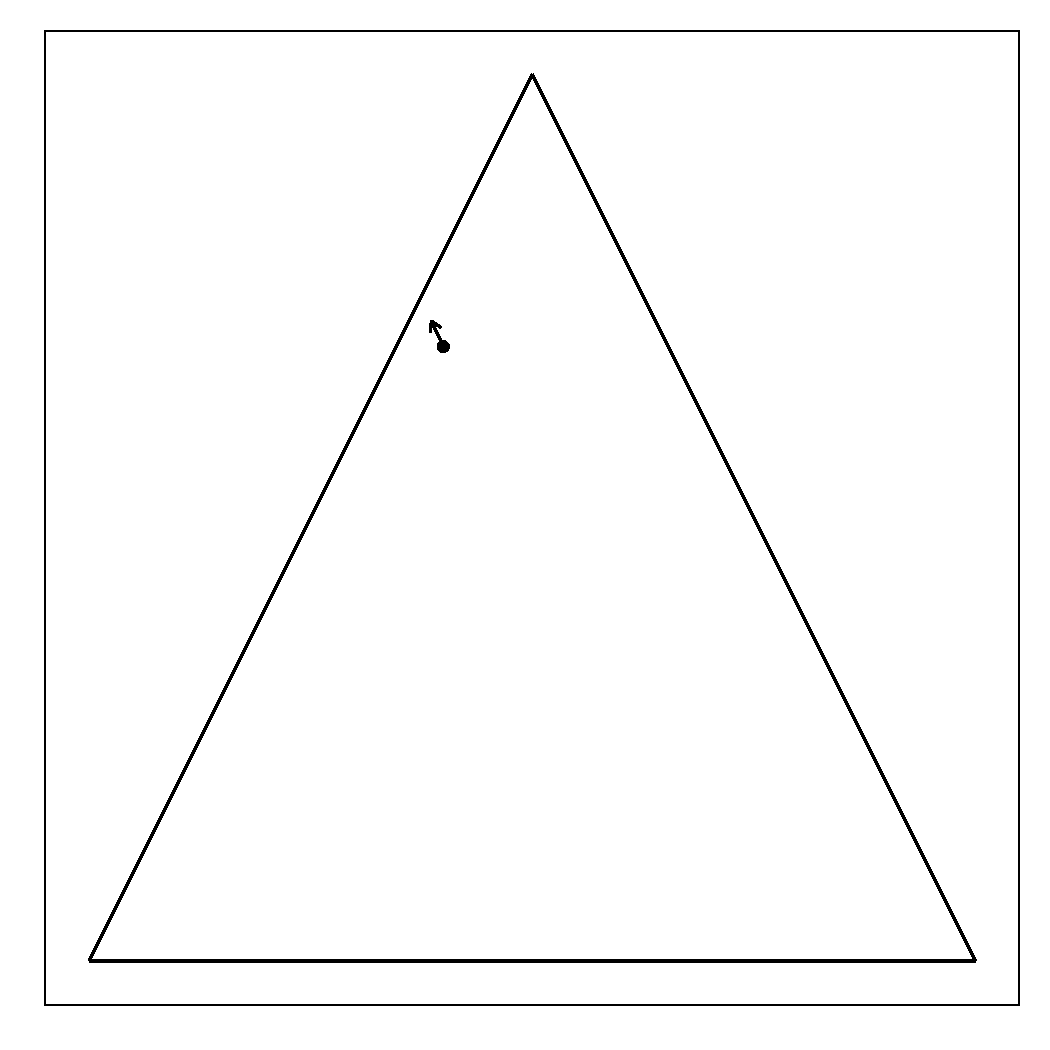
\includegraphics[width=\maxwidth]{figure/hitandrun_walkthrough2} 

\end{knitrout}

\caption{The function then chooses a random direction, as shown by the arrow.}
\end{figure}

\begin{figure}[H]
\begin{knitrout}
\definecolor{shadecolor}{rgb}{0.969, 0.969, 0.969}\color{fgcolor}
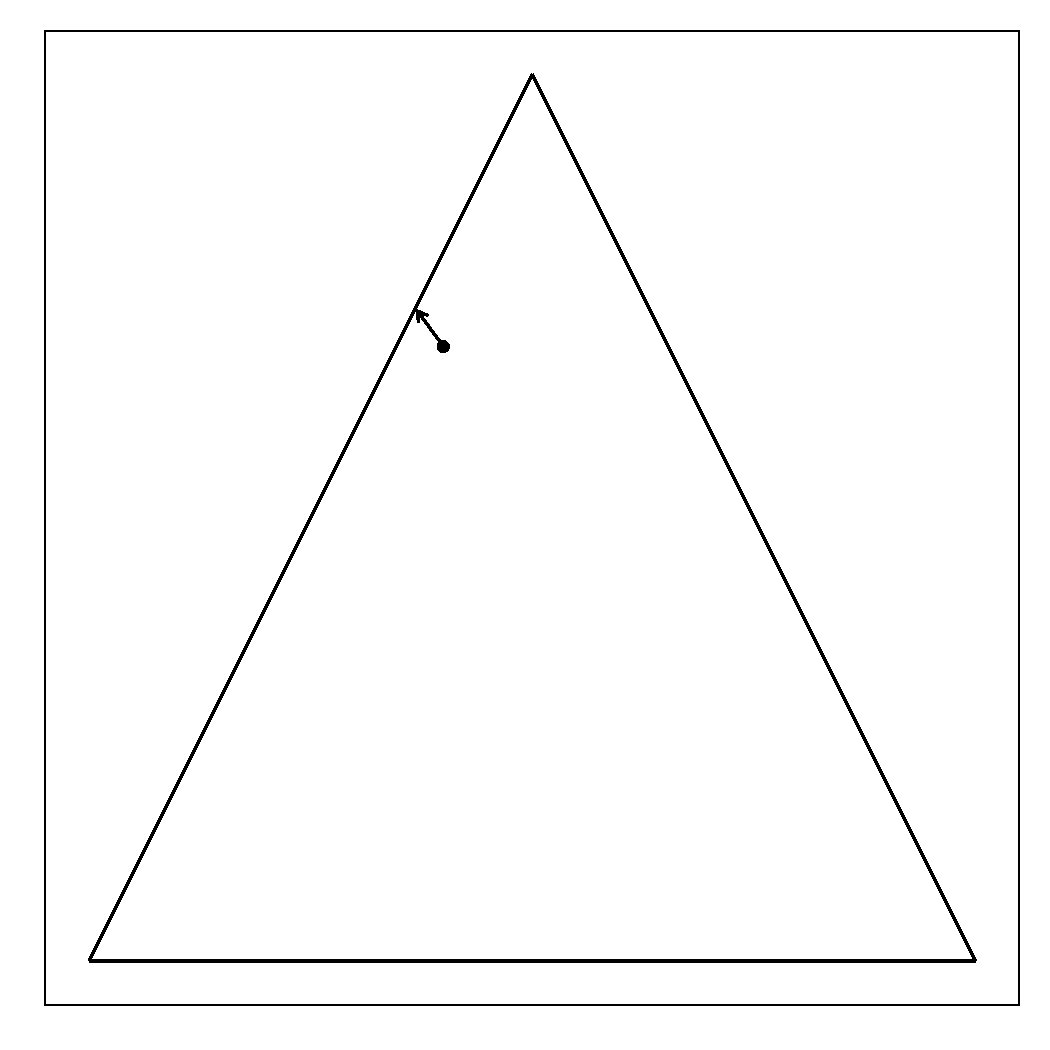
\includegraphics[width=\maxwidth]{figure/hitandrun_walkthrough3} 

\end{knitrout}

\caption{hitandrun() goes in the chosen direction until it hits an edge of the simplex. In this figure, the arrow was extended until it hit a wall.}
\end{figure}

\begin{figure}[H]
\begin{knitrout}
\definecolor{shadecolor}{rgb}{0.969, 0.969, 0.969}\color{fgcolor}
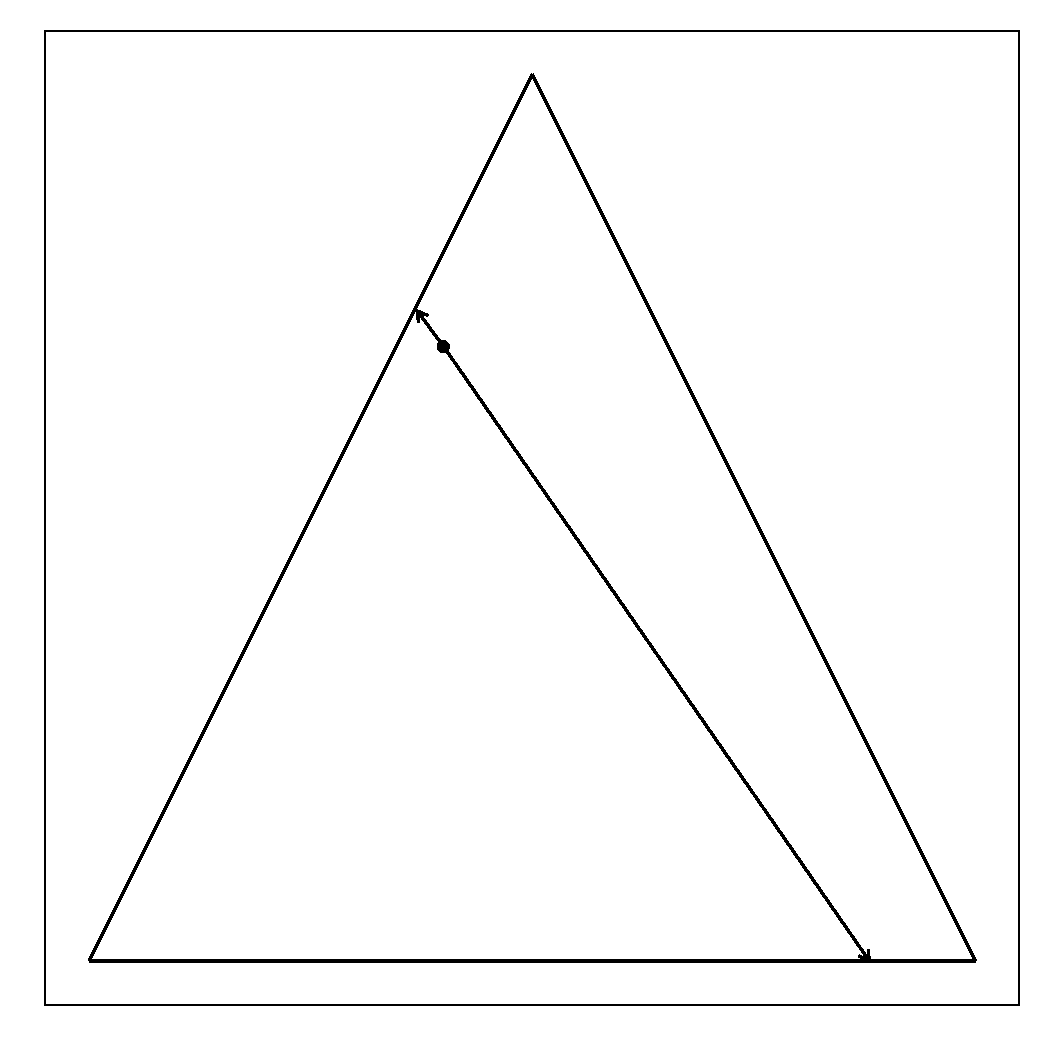
\includegraphics[width=\maxwidth]{figure/hitandrun_walkthrough4} 

\end{knitrout}

\caption{Next, hitandrun() goes in the negative direction until it hits another point on the edge of the simplex. This is shown with another arrow.}
\end{figure}

\begin{figure}[H]
\begin{knitrout}
\definecolor{shadecolor}{rgb}{0.969, 0.969, 0.969}\color{fgcolor}
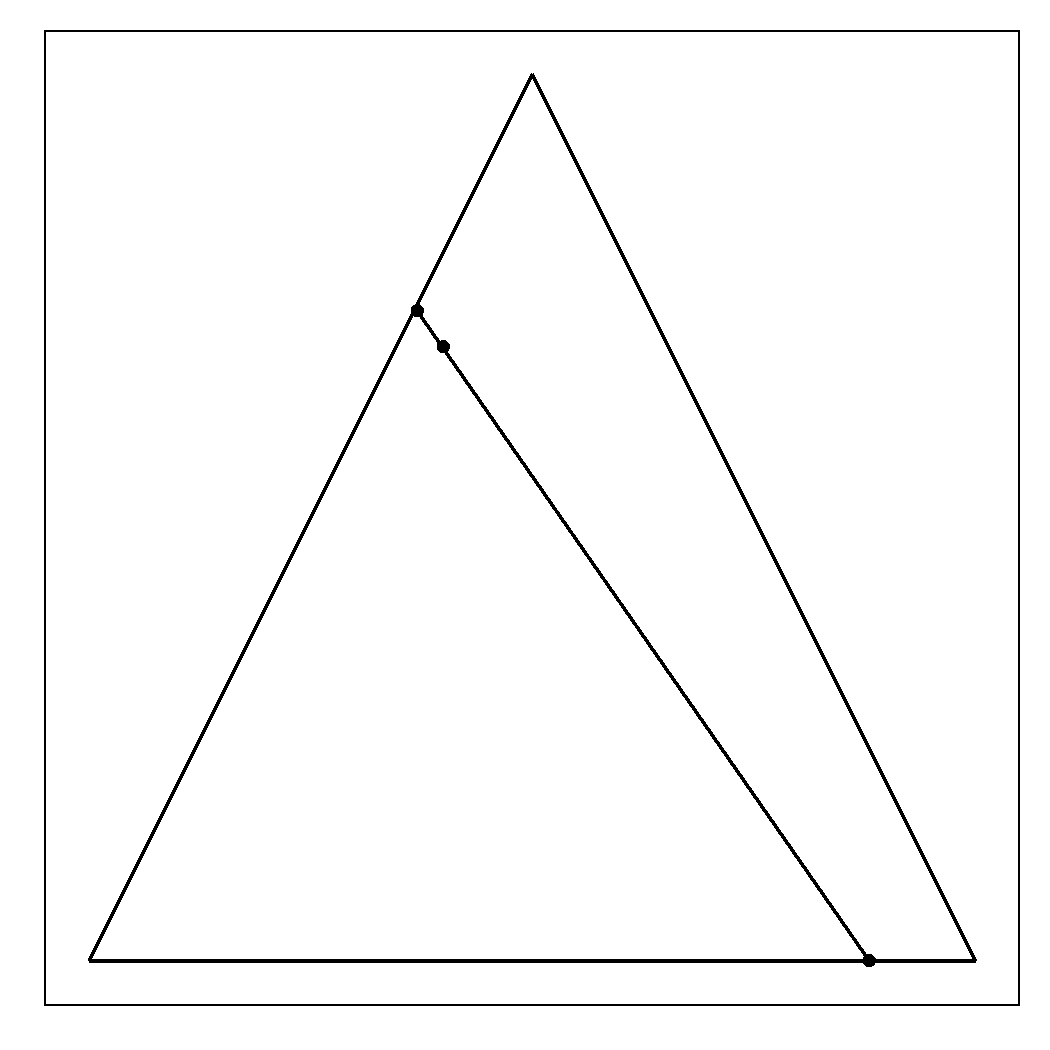
\includegraphics[width=\maxwidth]{figure/hitandrun_walkthrough5} 

\end{knitrout}

\caption{A line segment is formed. It passes through the initial point and connects the two points where the directional arrows intersected the simplex.}
\end{figure}

\begin{figure}[H]
\begin{knitrout}
\definecolor{shadecolor}{rgb}{0.969, 0.969, 0.969}\color{fgcolor}
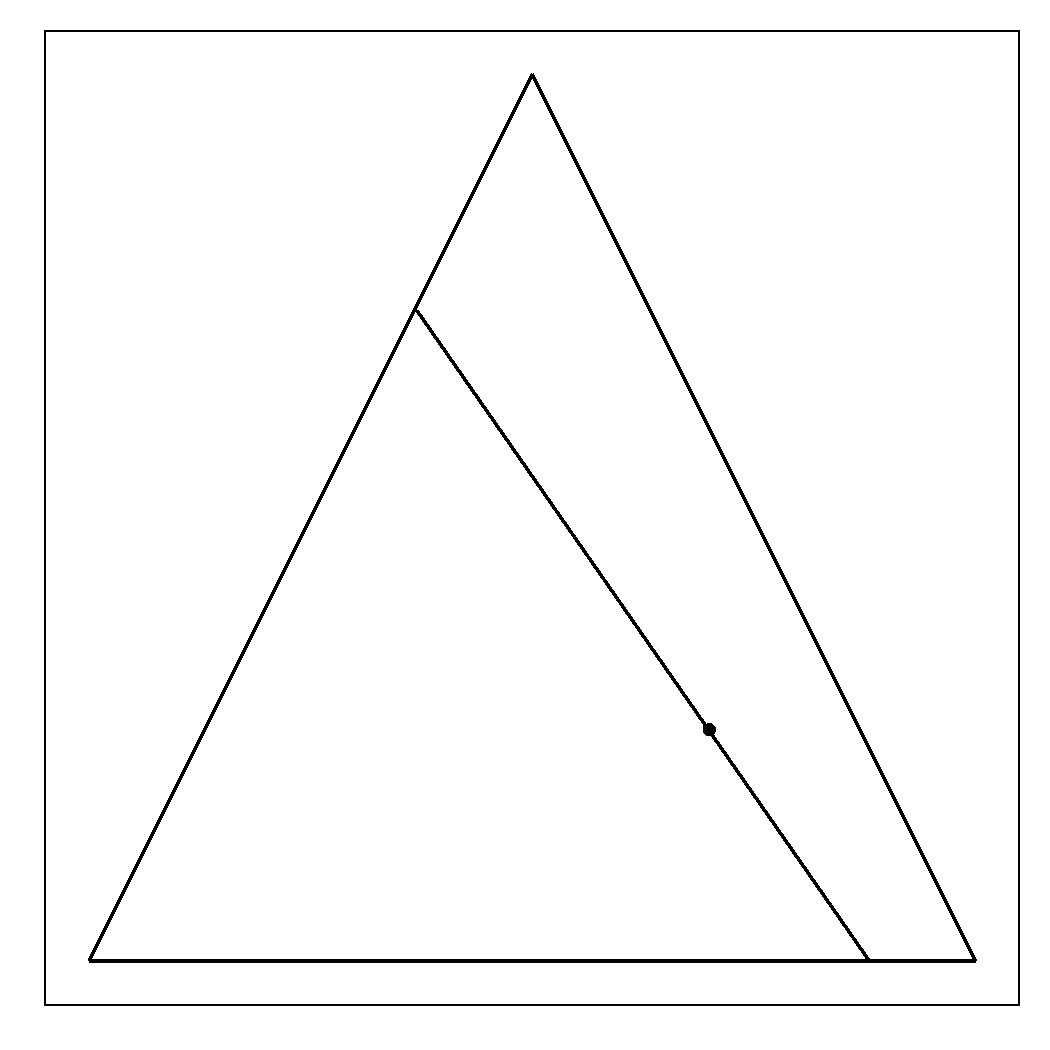
\includegraphics[width=\maxwidth]{figure/hitandrun_walkthrough6} 

\end{knitrout}

\caption{Finally, a random point is picked on the line segment shown in figure 10.}
\end{figure}

\begin{figure}[H]
\begin{knitrout}
\definecolor{shadecolor}{rgb}{0.969, 0.969, 0.969}\color{fgcolor}
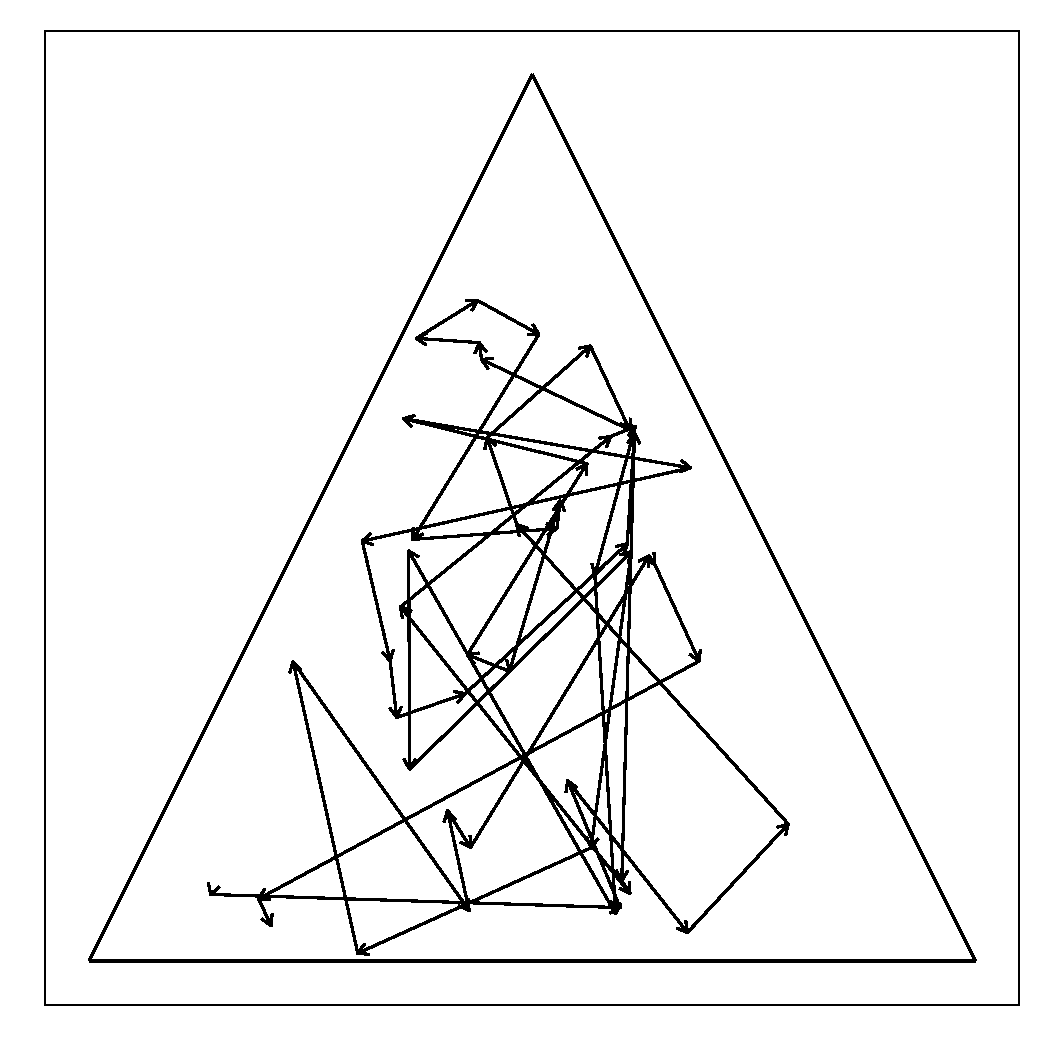
\includegraphics[width=\maxwidth]{figure/hitandrun_walkthrough7} 

\end{knitrout}

\caption{hitandrun() then repeats the previous steps, resulting in the creation of many randomized points. This figure displays the outcome of 50 repetitions of the hitandrun algorithm that was just explained.}
\end{figure}

\section*{mirror()}

mirror() is another function used in the process of creating random portfolios.This function also consists of points jumping from one random place to another.

\begin{figure}[H]
\begin{knitrout}
\definecolor{shadecolor}{rgb}{0.969, 0.969, 0.969}\color{fgcolor}
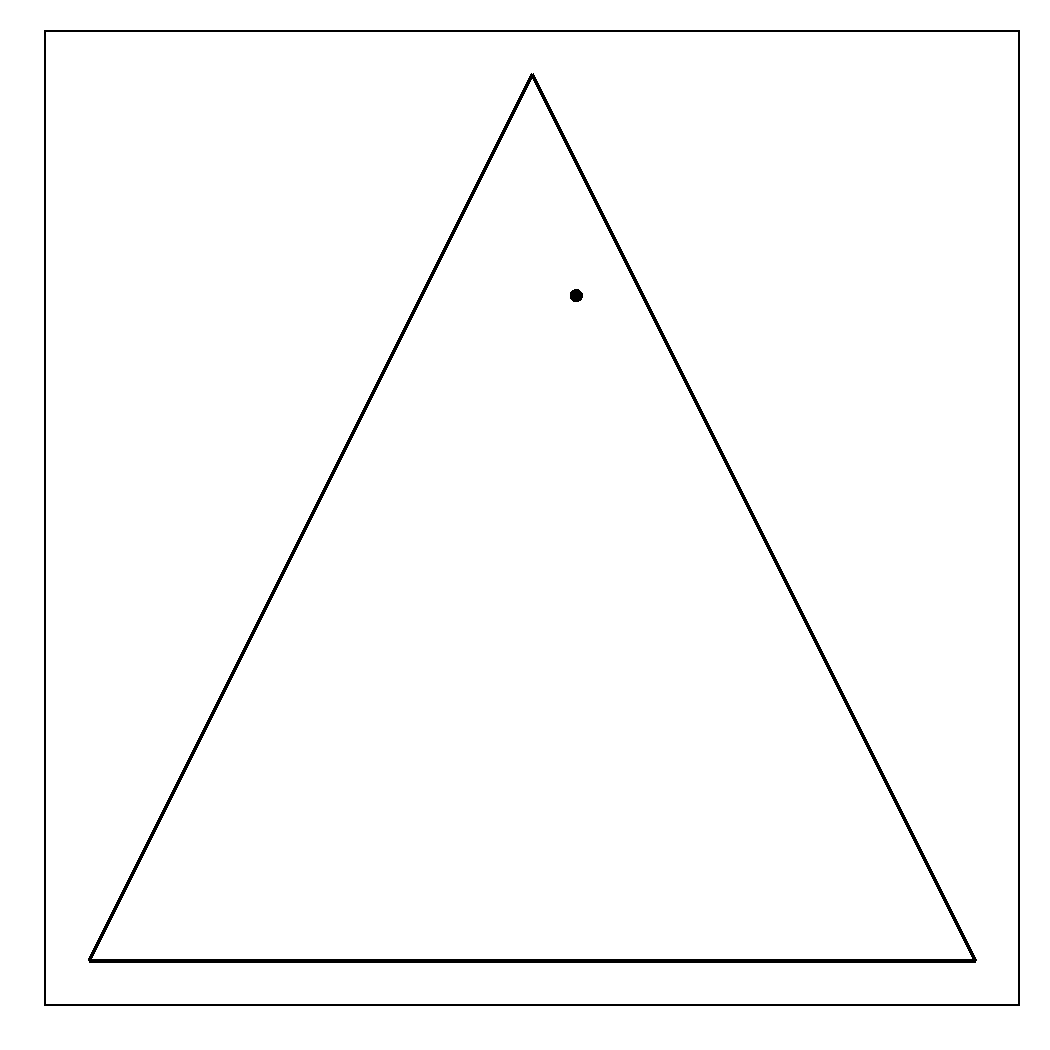
\includegraphics[width=\maxwidth]{figure/mirror_walkthrough1} 

\end{knitrout}

\caption{Similar to hitandrun(), mirror() begins by selecting a random point.}
\end{figure}

\begin{figure}[H]
\begin{knitrout}
\definecolor{shadecolor}{rgb}{0.969, 0.969, 0.969}\color{fgcolor}
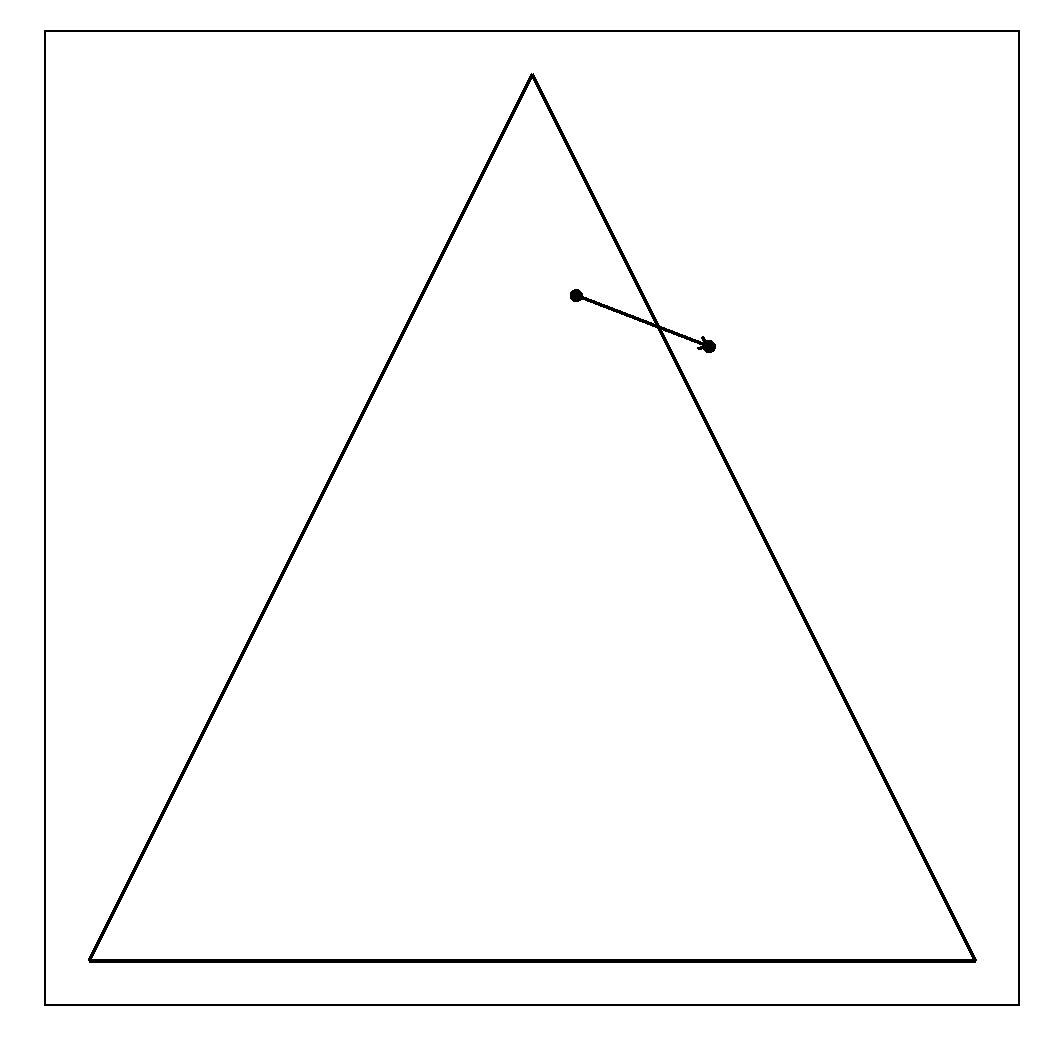
\includegraphics[width=\maxwidth]{figure/mirror_walkthrough2} 

\end{knitrout}

\caption{The point then jumps to a random place in space. It does not matter if that point is within or outside of the simplex.}
\end{figure}

\begin{figure}[H]
\begin{knitrout}
\definecolor{shadecolor}{rgb}{0.969, 0.969, 0.969}\color{fgcolor}
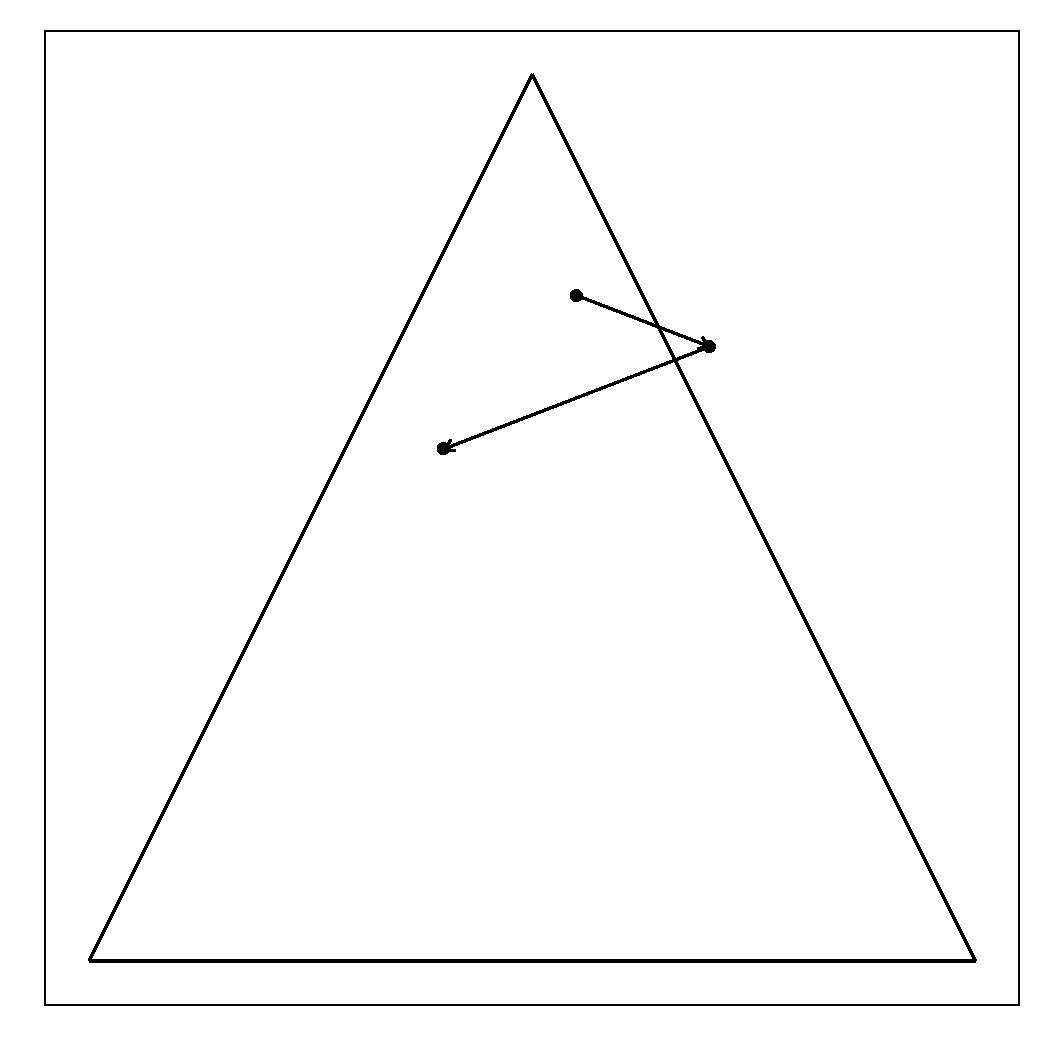
\includegraphics[width=\maxwidth]{figure/mirror_walkthrough3} 

\end{knitrout}

\caption{The step displayed in Figure 14 is then repeated.}
\end{figure}

\end{document}

\begin{knitrout}
\definecolor{shadecolor}{rgb}{0.969, 0.969, 0.969}\color{fgcolor}\begin{kframe}


{\ttfamily\noindent\bfseries\color{errorcolor}{\#\# Error: object '.x37' not found}}\end{kframe}
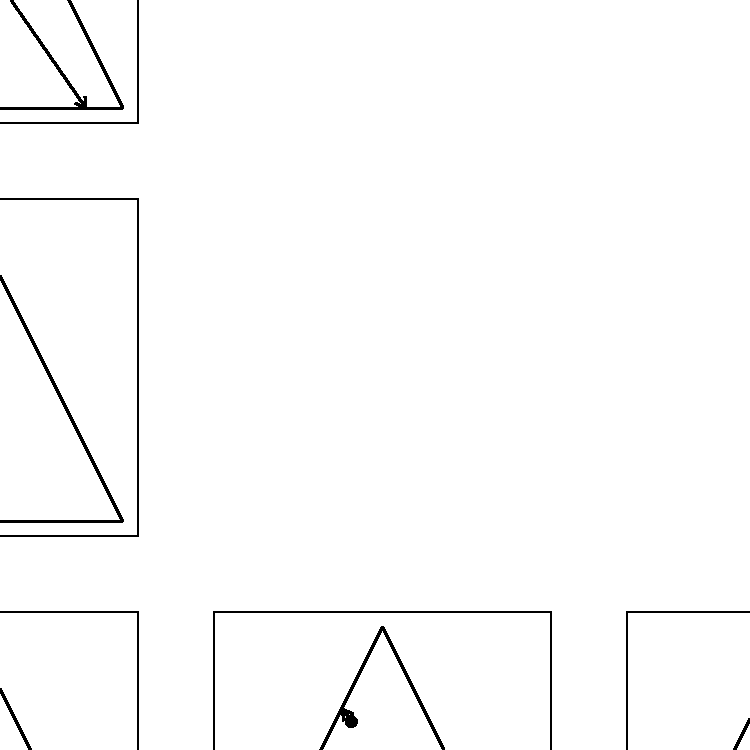
\includegraphics[width=\maxwidth]{figure/hitandrun_walkthrough} 

\end{knitrout}


